\documentclass[handout]{beamer}

\usepackage[utf8]{inputenc} % Language and font encoding
\usepackage[icelandic]{babel}
\usepackage[T1]{fontenc}


\usepackage{tikz}
\usepackage[listings,theorems]{tcolorbox}
\usepackage{booktabs}
\usepackage{minted} %Minted and configuration
\usemintedstyle{default}

\renewcommand{\theFancyVerbLine}{\sffamily \arabic{FancyVerbLine}}
%%%%%%%%%%%
% More math
%%%%%%%%%%%
\newcommand{\Mod}[1]{\ \text{mod}\ #1}

%%%%%%%%%%%%%%%%%%%%%%
% Beamer configuration
%%%%%%%%%%%%%%%%%%%%%%
\setbeamertemplate{navigation symbols}{}
\usecolortheme{dove}
\setbeamercolor{frametitle}{fg=white}

\usebackgroundtemplate%
{%
\vbox to \paperheight{

\includegraphics[width=\paperwidth]{Pics/hi-slide-head-2016}

\vfill
\hspace{0.5cm}
\includegraphics[width=0.3\paperwidth]{Pics/hi-von-logo}
\vspace{0.4cm}
    }%
}

\AtBeginSection[]
{
  \begin{frame}<beamer>
    \frametitle{Yfirlit}
    \tableofcontents[currentsection]
  \end{frame}
}

\setbeamerfont{frametitle}{size=\normalsize}
\addtobeamertemplate{frametitle}{}{\vspace*{0.5cm}}

%%%%%%%%%%%%%%%%%%%%%%%%%
% tcolorbox configuration
%%%%%%%%%%%%%%%%%%%%%%%%%

% Setup from: http://tex.stackexchange.com/a/43329/21638
\tcbset{%
    noparskip,
    colback=gray!10, %background color of the box
    colframe=gray!40, %color of frame and title background
    coltext=black, %color of body text
    coltitle=black, %color of title text 
    fonttitle=\bfseries,
    alerted/.style={coltitle=red, colframe=gray!40},
    example/.style={coltitle=black, colframe=green!20, colback=green!5},
}


%%%%%%%%%%%%%%%%%%%%%%%
% Further configuration
%%%%%%%%%%%%%%%%%%%%%%%
\hypersetup{colorlinks=true,pdfauthor={Eirikur Ernir Thorsteinsson},linkcolor=blue,urlcolor=blue}
\graphicspath{{./Pics/}}

\author{Eiríkur Ernir Þorsteinsson}
\institute{Háskóli Íslands}
\date{Haust 2016}

\title{Stærðfræðimynstur í tölvunarfræði}
\subtitle{Vika 2, seinni fyrirlestur}

\begin{document}

\begin{frame}
\titlepage
\end{frame}

\section{Inngangur}

\begin{frame}{Í síðasta tíma}
\begin{itemize}
 \item Mengi!
 \begin{itemize}
  \item Stök í mengjum
  \item Hlutmengi
  \item Veldismengi og mengjamargfeldi
  \item Sniðmengi og sammengi
 \end{itemize}
\end{itemize}
\end{frame}

\section{Föll}

\begin{frame}{Föll}
\begin{itemize}
 \item Fall er hugtak sem er mörgum kunnuglegt úr stærðfræðigreiningu
 \begin{itemize}
  \item $f(x) = x^2$ er fall
  \item $\sin(x)$ er fall
 \end{itemize}
 \item Oftast hefur verið um að ræða föll sem taka inn eina rauntölu og skila annarri rauntölu
 \begin{itemize}
  \item Við notum opnari skilgreiningu
 \end{itemize}
\end{itemize}
\end{frame}

\begin{frame}{Skilgreining á falli}
\begin{tcolorbox}[title=Fall]
Látum $A$ og $B$ vera mengi sem eru ekki tóm. Fall (e. \emph{function}) $f$ frá $A$ til $B$ er ákvörðun á nákvæmlega einu staki í $B$ fyrir sérhvert stak í $A$.

Við skrifum $f(a) = b$ þegar $b$ er stakið sem fallið $f$ ákvarðar fyrir stakið $a$.

Við skrifum $f: A \to B$ þegar $f$ er fall frá $A$ til $B$.
\end{tcolorbox}

Föll eru líka kölluð varpanir (e. \emph{mapping} eða \emph{transformation}). Fall $f: A \to B$ varpar stökum úr mengi $A$ yfir í mengi $B$.
\end{frame}

\begin{frame}{Dæmi um föll}
\begin{itemize}
 \item Föll sem skilgreind eru með formúlu, föll með þekkt nöfn
 \begin{itemize}
  \item $f(x) = x^2$ er $\mathbf{R} \to \mathbf{R}$
  \item $\sin(x)$ er líka $\mathbf{R} \to \mathbf{R}$
 \end{itemize}
 \item Ákvörðun einkunna í þessu námskeiði má tákna með falli
 \item Ákvörðun nafna út frá kennitölum má tákna með falli \pause
 \begin{itemize}
  \item Ákvörðun kennitala út frá nöfnum er ekki fall!
 \end{itemize}
\end{itemize}
\end{frame}

\begin{frame}{Formengi og bakmengi}
\begin{tcolorbox}[title=Formengi og bakmengi]
Sé $f$ fall frá $A$ til $B$ kallast $A$ formengi (e. \emph{domain}) fallsins og $B$ bakmengi (e. \emph{codomain}) þess. Sé $f(a) = b$ er sagt að $b$ sé mynd (e. \emph{image}) $a$ og að $a$ sé formynd (e. \emph{preimage}) $a$.
\end{tcolorbox}
Sum föll eru hlutskilgreind (e. \emph{partial functions}), þ.e.a.s. að þau eru ekki skilgreind fyrir öll stök í formengi sínu. Dæmi: $f(x) = 1/x$.
\end{frame}

\begin{frame}[fragile]{Föll í forritun}
\begin{itemize}
 \item Föll eru gríðarlega mikið notuð í forritun, í ýmsum myndum
 \begin{itemize}
  \item Dæmigert fall í forritun:
  \begin{itemize}
   \item Tekur inn breytur
   \item Framkvæmir reikniaðgerðir
   \item Skilar niðurstöðu í samræmi við inntakið 
  \end{itemize}
 \end{itemize}
 \item Í mörgum forritunarmálum eru formengi og bakmengi tilgreind þegar fall er skilgreint
\end{itemize}
\begin{minted}[frame=lines]{java}
// Fall frá mengi strengja til mengi heiltalna
public static int f (String s) {
  ...
}
\end{minted}

\end{frame}

\begin{frame}{Eintæk föll}
\begin{tcolorbox}[title=Eintækt fall]
Fall er eintækt (e. \emph{injective}) ef það varpar engum tveimur stökum í formengi sínu í sama stak bakmengisins, þ.e.a.s. ef \[\forall a \forall b (f(a) = f(b) \to a = b)\] og þar með \[\forall a \forall b (f(a) \neq f(b) \to a \neq b)\].
\end{tcolorbox}
\end{frame}

\begin{frame}{Átæk föll}
\begin{tcolorbox}[title=Átækt fall]
Fall $f$ er átækt (e. \emph{surjective}) ef það ``þekur'' bakmengi sitt, þ.e.a.s. að fyrir hvert stak $b$ í bakmenginu er til stak í formenginu $a$ svo að $f(a) = b$, \[\forall b \exists a (f(a) = b)\].
\end{tcolorbox}
\end{frame}

\begin{frame}{Eintækni og átækni}
\begin{center}
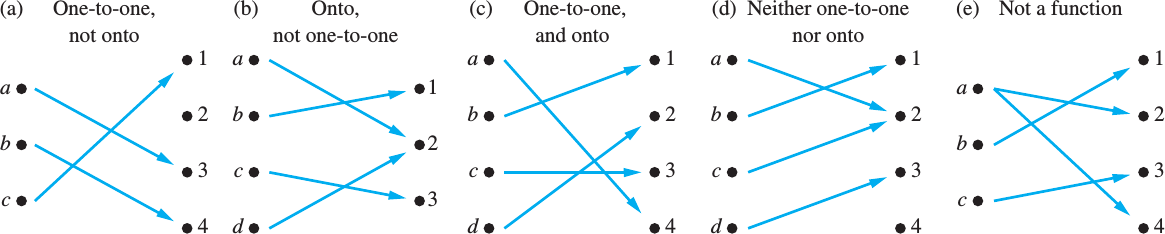
\includegraphics[width=\textwidth]{function-types}
\end{center}
Fall sem er bæði eintækt og átækt er kallað gagntækt (e. \emph{bijective}).
\end{frame}

\begin{frame}{Andhverfanleg föll}
\begin{tcolorbox}[title=Andhverfanlegt fall]
Látum $f$ vera gagntækt fall frá $A$ til $B$. Þá er andhverfa fallsins $f$ fallið sem varpar $b \in B$ í stakið $a \in A$ sem um gildir að $f(a) = b$.

Andhverfa fallsins $f$ er táknuð með $f^{-1}$. Um $f^{-1}$ gildir:

\[
 f(a) = b \equiv f^{-1}(b) = a
\]

\end{tcolorbox}
Fall sem er ekki gagntækt er óandhverfanlegt. Hægt er að búa til andhverfanlegt fall úr óandhverfanlegu með því að takmarka formengi þess.
\end{frame}

\begin{frame}{Samantekt}
\begin{itemize}
 \item Látum $f: A \to B$
 \begin{itemize}
  \item Til að sýna að fall sé eintækt: Sýna að $f(x) = f(y)$ fyrir ótilgreind $x, y \in A$ þegar $x \neq y$.
  \item Til að sýna að fall sé átækt: Athuga ótilgreint $y \in B$ og finna $x \in A$ svo að $f(x) = y$
 \end{itemize}
 \item Til að sýna fram á hið gagnstæða, finnið mótdæmi
\end{itemize}

\end{frame}


\begin{frame}{Samskeyting falla}
\begin{tcolorbox}[title=Samskeyting falla]
Látum $g$ vera fall frá menginu $A$ til mengisins $B$ og látum $f$ vera fall frá menginu $B$ til mengisins $C$. Samskeyting (e. \emph{composition}) fallanna $f$ og $g$, fyrir $a \in A$ er þá táknuð með $f \circ g$ og skilgreinist af

\[
 (f \circ g)(a) = f(g(a))
\]

\end{tcolorbox}
Oft er hægt að einfalda föll með því að skrifa þau sem samskeytingar. Við forritun kemur þetta sérstaklega við í fallsforritunarmálum og skeljaskipunum.
\end{frame}

\section{Fylki}

\begin{frame}{Fylki}
\begin{tcolorbox}[title=Fylki]
Fylki (e. \emph{matrix}) er ferhyrnt safn af tölum sem raðast í línur og dálka. Fylki með $m$ línum og $n$ dálkum er kallað $m \times n$ fylki.
\end{tcolorbox}
Fylki og aðgerðir á þau koma mikið við sögu í forritun sem tengist vísindalegum útreikningum og í tölvugrafík.

Dæmi um fylki: Fylkið
\[
\begin{bmatrix}
1&1\\0&2\\1&4
\end{bmatrix}
\]
er $3 \times 2$ fylki.
\end{frame}

\begin{frame}{Fylkjamargföldun}
Hægt er að skilgreina margar reikniaðgerðir fyrir fylki. Aðgerð sem oft kemur við sögu er fylkjamargföldun.

\begin{tcolorbox}[title=Fylkjamargföldun]
Látum $A$ vera $m \times k$ fylki og $B$ vera $k \times n$ fylki. Margfeldi $A$ og $B$, táknað með $AB$, er $m \times n$ fylki þar sem stak $i, j$ er summa margfelda staka úr $i$-tu línu $A$ og $j$-ta dálks $B$. Þ.e.a.s. fyrir stak $c_{ij}$ í $AB$ gildir:

\[
 c_{ij} = a_{i1}b_{1j} + a_{i2}b_{2j} + \ldots + a_{ij}b_{kj}
\]
\end{tcolorbox}
\end{frame}

\begin{frame}{Fylkjamargföldun - dæmi}
\[
\begin{bmatrix}
1&0&4\\2&1&1\\3&1&0\\0&2&2
\end{bmatrix}
\begin{bmatrix}
2&4\\
1&1\\
3&0\\
\end{bmatrix}
=
\begin{bmatrix}
14&4\\
8&9\\
7&13\\
8&2\\
\end{bmatrix}
\]

\end{frame}


\section{Runur og rakningarvensl}

\begin{frame}{Runur}
\begin{tcolorbox}[title=Runur]
Runa (e. \emph{sequence}) er fall frá hlutmengi heiltalna (oftast mengi jákvæðra heiltalna) til annars mengis $S$. Mynd heiltölunnar $n$ er táknuð með $a_n$. Sagt er að $a_n$ sé liður (e. \emph{term}) í rununni.
\end{tcolorbox}
Bókin táknar runur með slaufusvigum, t.d. $\{a_n\}$. Runur eru samt ekki mengi.

Dæmi um runu:
\[
 \{a_n\} = a_1, a_2, a_3 \ldots = 1, \frac{1}{2}, \frac{1}{3}
\]
\[
 a_n = \frac{1}{n}
\]
\end{frame}

\begin{frame}[fragile]{Strengir}
\begin{itemize}
 \item Sérstök, mikið notuð gerð af runum kallast strengur (e. \emph{string})
 \item Strengur er endanleg runa af stöfum, úr endanlegu mengi (stafrófinu)
 \begin{itemize}
  \item Stafrófið getur verið hvaða mengi sem er, en algeng stafróf eru \texttt{\{'a', 'b', 'c', \ldots\}} og \texttt{\{0, 1\}}
 \end{itemize}
\end{itemize}

\begin{minted}[frame=lines]{java}
// Gagnagerðin String í Java í notkun
String s = "Ég er strengur!";
String b = "01010110";
\end{minted}
\end{frame}

\begin{frame}{Rakningarvensl}
\begin{tcolorbox}[title=Rakningarvensl]
Rakningarvensl (e. \emph{recurrence relation}) fyrir runu $\{a_n\}$ er jafna sem skilgreinir $a_n$ sem fall af einum eða fleiri fyrri liðum rununnar, þ.e.a.s. $a_0, a_1, \ldots, a_{n-1}$ fyrir öll $n > n_0$, þar sem $n_0$ er ekki-neikvæð heiltala.
\end{tcolorbox}
Runa er lausn (e. \emph{solution}) á rakningarvenslum ef liðir hennar uppfylla venslin. Liðirnir sem eru fyrir framan fyrsta liðinn sem rankningarvenslin tilgreina eru upphafsskilyrði (e. \emph{initial conditions}) þeirra.
\end{frame}

\begin{frame}{Dæmi um rakningarvensl}
Látum $\{a_n\}$ vera runu sem uppfyllir $a_n = a_{n-1} + 3$ fyrir $n=1, 2, 3, \ldots$ og setjum $a_0 = 2$. Hvað eru þá $a_1, a_2$ og $a_3$? \pause

\begin{align*}
a_1 &= a_0 + 3 = 2 + 3 = 5\\
a_2 &= 5 + 3 = 8\\
a_3 &= 8 + 3 = 11\\
\end{align*}

\end{frame}

\begin{frame}{Dæmi um rakningarvensl}
\begin{itemize}
 \item Fibonacci-rununa $f_0, f_1, f_2, \ldots$ má skilgreina með rakningavenslum
 \begin{itemize}
  \item Upphafsskilyrði: $f_0 = 0, f_1 = 1$
  \item Rakningavensl: $f_n = f_{n-1} + f_{n-2}$
 \end{itemize}
\end{itemize}
\end{frame}

\begin{frame}{Að leysa rakningarvensl}
\begin{itemize}
 \item Oft er nauðsynlegt að finna formúlu fyrir liði runu sem skilgreind er með rakningarvenslum
 \item Formúlan er sögð vera á lokuðu sniði (e. \emph{closed form}) ef hún inniheldur einungis ``einfaldar'' grunnaðgerðir og föll
 \item Algengt: Giska á rétta formúlu, sem síðan er sannreynd með þrepun (e. \emph{induction})
 \begin{itemize}
  \item Gerum líklega meira af því síðar
 \end{itemize}
\end{itemize}
\end{frame}


\section{Fjöldatölur og reiknanleiki}

\begin{frame}{Fjöldatölur}
Við höfum áður kynnst fjöldatölum. Útvíkkum nú hugtakið:

\begin{tcolorbox}[title=Eins fjöldatölur]
Mengin $A$ og $B$ hafa sömu fjöldatölu ef til er gagntækt fall frá $A$ til $B$.
\end{tcolorbox}

Þá má einnig skilgreina:

\begin{tcolorbox}[title=Teljanleiki]
Mengi sem er endanlegt eða hefur sömu fjöldatölu og mengi jákvæðra heiltalna er teljanlegt (e. \emph{countable}). Þegar óendanlegt mengi $S$ er teljanlegt skilgreinum við fjöldatölu þess sem $|S| = \aleph_0$.
\end{tcolorbox}
\end{frame}

\begin{frame}{Reiknanleiki}
\begin{itemize}
 \item Til að fall sé reiknanlegt (e. \emph{computable}) þarf að vera til forrit í einhverju forritunarmáli sem finnur gildi þess
 \item Til eru óreiknanleg föll!
 \item Þekkt atriði:
 \begin{itemize}
  \item Fjöldi forrita er teljanlega óendanlegur
  \item Fjöldi falla frá teljanlega óendanlegu mengi yfir í sjálft sig er óteljanlegur
 \end{itemize}
\end{itemize}
\end{frame}

\begin{frame}{Næst}
Reiknirit (kafli 3.1) og vöxtur falla (kafli 3.2)
\end{frame}


\end{document}
